\begin{figure}[!h]
\centering
\resizebox{\textwidth}{!}{%
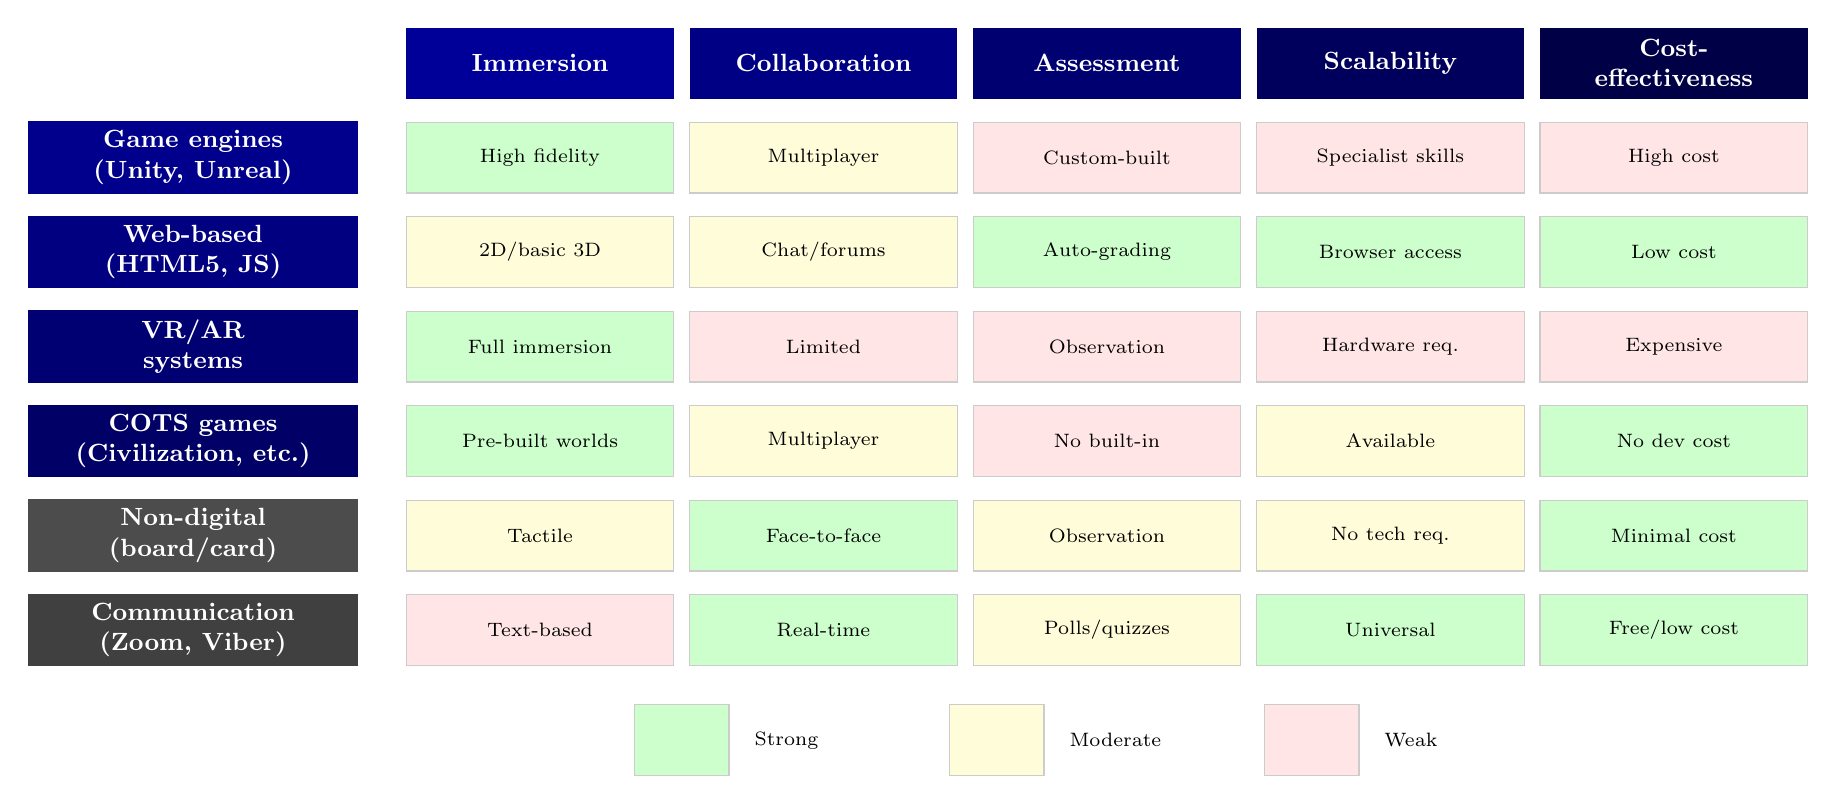
\begin{tikzpicture}[
  hdr/.style={font=\small\bfseries, text=white, minimum height=0.9cm,
    minimum width=3.4cm, align=center},
  rhdr/.style={font=\small\bfseries, text=white, minimum height=0.9cm,
    minimum width=4.2cm, align=center, anchor=east},
  cell/.style={rectangle, draw=gray!40, minimum height=0.9cm,
    minimum width=3.4cm, align=center, font=\scriptsize},
  strong/.style={cell, fill=green!20},
  moderate/.style={cell, fill=yellow!15},
  weak/.style={cell, fill=red!10},
]

% Column headers
\node[hdr, fill=blue!60!black] at (0, 0) {Immersion};
\node[hdr, fill=blue!52!black] at (3.6, 0) {Collaboration};
\node[hdr, fill=blue!44!black] at (7.2, 0) {Assessment};
\node[hdr, fill=blue!36!black] at (10.8, 0) {Scalability};
\node[hdr, fill=blue!28!black] at (14.4, 0) {Cost-\\effectiveness};

% Row 1: Game engines (Unity, Unreal)
\node[rhdr, fill=blue!55!black] at (-2.3, -1.2) {Game engines\\(Unity, Unreal)};
\node[strong] at (0, -1.2) {High fidelity};
\node[moderate] at (3.6, -1.2) {Multiplayer};
\node[weak] at (7.2, -1.2) {Custom-built};
\node[weak] at (10.8, -1.2) {Specialist skills};
\node[weak] at (14.4, -1.2) {High cost};

% Row 2: Web-based (HTML5, JS)
\node[rhdr, fill=blue!50!black] at (-2.3, -2.4) {Web-based\\(HTML5, JS)};
\node[moderate] at (0, -2.4) {2D/basic 3D};
\node[moderate] at (3.6, -2.4) {Chat/forums};
\node[strong] at (7.2, -2.4) {Auto-grading};
\node[strong] at (10.8, -2.4) {Browser access};
\node[strong] at (14.4, -2.4) {Low cost};

% Row 3: VR/AR systems
\node[rhdr, fill=blue!45!black] at (-2.3, -3.6) {VR/AR\\systems};
\node[strong] at (0, -3.6) {Full immersion};
\node[weak] at (3.6, -3.6) {Limited};
\node[weak] at (7.2, -3.6) {Observation};
\node[weak] at (10.8, -3.6) {Hardware req.};
\node[weak] at (14.4, -3.6) {Expensive};

% Row 4: COTS games (Civilization, etc.)
\node[rhdr, fill=blue!40!black] at (-2.3, -4.8) {COTS games\\(Civilization, etc.)};
\node[strong] at (0, -4.8) {Pre-built worlds};
\node[moderate] at (3.6, -4.8) {Multiplayer};
\node[weak] at (7.2, -4.8) {No built-in};
\node[moderate] at (10.8, -4.8) {Available};
\node[strong] at (14.4, -4.8) {No dev cost};

% Row 5: Non-digital (board/card)
\node[rhdr, fill=gray!60!black] at (-2.3, -6.0) {Non-digital\\(board/card)};
\node[moderate] at (0, -6.0) {Tactile};
\node[strong] at (3.6, -6.0) {Face-to-face};
\node[moderate] at (7.2, -6.0) {Observation};
\node[moderate] at (10.8, -6.0) {No tech req.};
\node[strong] at (14.4, -6.0) {Minimal cost};

% Row 6: Communication platforms (Zoom, Viber)
\node[rhdr, fill=gray!50!black] at (-2.3, -7.2) {Communication\\(Zoom, Viber)};
\node[weak] at (0, -7.2) {Text-based};
\node[strong] at (3.6, -7.2) {Real-time};
\node[moderate] at (7.2, -7.2) {Polls/quizzes};
\node[strong] at (10.8, -7.2) {Universal};
\node[strong] at (14.4, -7.2) {Free/low cost};

% Legend
\node[strong, minimum width=1.2cm] at (1.8, -8.6) {};
\node[font=\scriptsize, anchor=west] at (2.6, -8.6) {Strong};
\node[moderate, minimum width=1.2cm] at (5.8, -8.6) {};
\node[font=\scriptsize, anchor=west] at (6.6, -8.6) {Moderate};
\node[weak, minimum width=1.2cm] at (9.8, -8.6) {};
\node[font=\scriptsize, anchor=west] at (10.6, -8.6) {Weak};

\end{tikzpicture}%
}% end resizebox
\caption{Platform type--pedagogical affordance alignment matrix. Green indicates strong alignment, yellow moderate, red weak. No single platform excels across all dimensions, suggesting that multi-platform designs may be necessary for comprehensive gamification.}
\label{fig:platform-pedagogy-matrix}
\end{figure}
